\section{Istruzioni all'uso}
\subsection{Pagine User}
In questa Sezione mostriamo le pagine riservate all'utente.
\subsubsection{Landing page}
All'avvio del prodotto verrà visualizzata la landing page, che presenta il logo dell'assistente virtuale e un messaggio di benvenuto. In questa fase, l'utente può scegliere di accedere al sistema.
\begin{figure}[h!]
    \centering
    \includegraphics[width=0.8\textwidth]{./img/landingPage.png}
    \caption{Schermata della landing page}
\end{figure}

\subsubsection{Pagina di Accesso}
Cliccando sul bottone blu si passerà direttamente alla pagina di accesso, dove l'utente dovrà inserire le proprie credenziali (\textit{username} e \textit{password}) per autenticarsi.
\begin{figure}[h!]
    \centering
    \includegraphics[width=0.8\textwidth]{./img/paginaAccesso.png}
    \caption{Schermata della pagina di accesso}
\end{figure}

\subsubsection{Pagina di Registrazione}
Nel caso in cui non si possieda un account, è possibile registrarsi dalla pagina di registrazione cliccando sul link presente nella pagina di autenticazione.
Qui l'utente dovrà inserire i campi obbligatori \{ \textit{username; password; email; nome; cognome} \} e volendo opzionalmente può inserire il numero di telefono.
\begin{figure}[h!]
    \centering
    \includegraphics[width=0.8\textwidth]{./img/paginaRegistrazione.png}
    \caption{Schermata della pagina di registrazione}
\end{figure}

\subsubsection{Schermata iniziale}
Una volta effettuato l'accesso verremo accolti da questa Schermata iniziale composta da 3 elementi, una navbar superiore, una navbar laterale e il contenuto della pagina. Da qui è possibile iniziare una conversazione mettendo il titolo della conversazione e schiacciando il bottone: "inizia la conversazione".
\begin{figure}[h!]
    \centering
    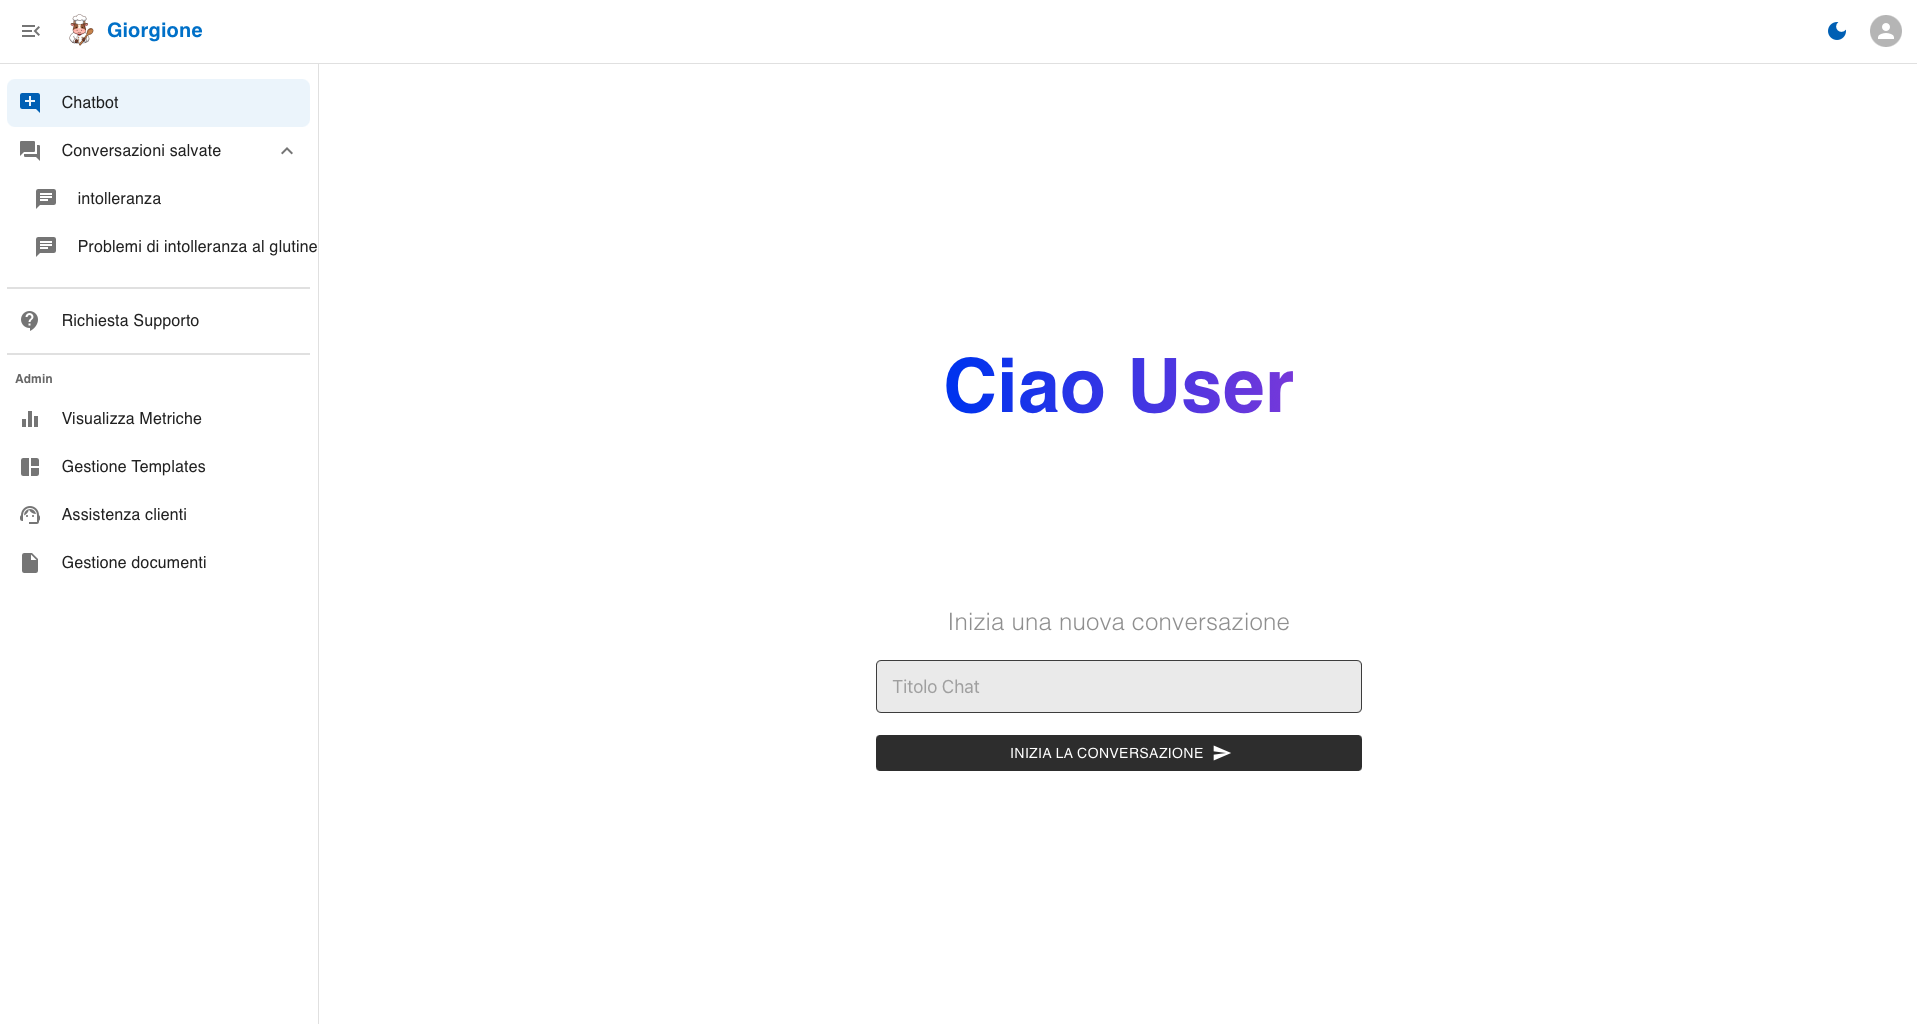
\includegraphics[width=0.8\textwidth]{./img/paginaIniziale.png}
    \caption{Schermata della pagina di registrazione}
\end{figure}

\subsubsection{Schermata di conversazione}
Una volta creata la conversazione dalla schermata iniziale l'utente può andare nel menù laterale (\textit{nel caso esso sia chiuso si può aprire tramite menù ad hamburger}) e selezionare la voce: "\textit{Conversazioni salvate}" che aprirà un menù a tendina dove l'utente potrà selezionare la conversazione desiderata.
\begin{figure}[h!]
    \centering
    \begin{subfigure}{0.3\textwidth}
        \centering
        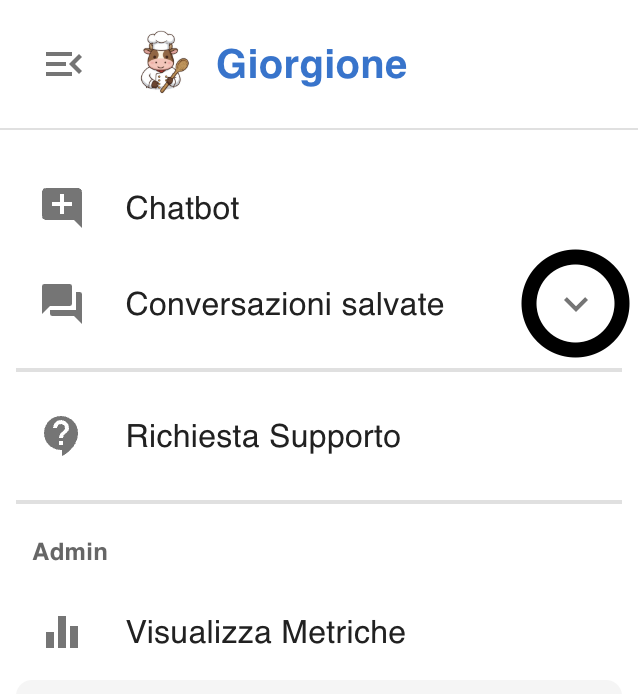
\includegraphics[width=\textwidth]{./img/laterale1.png}
    \end{subfigure}
    \hspace{0.05\textwidth}
    \begin{subfigure}{0.3\textwidth}
        \centering
        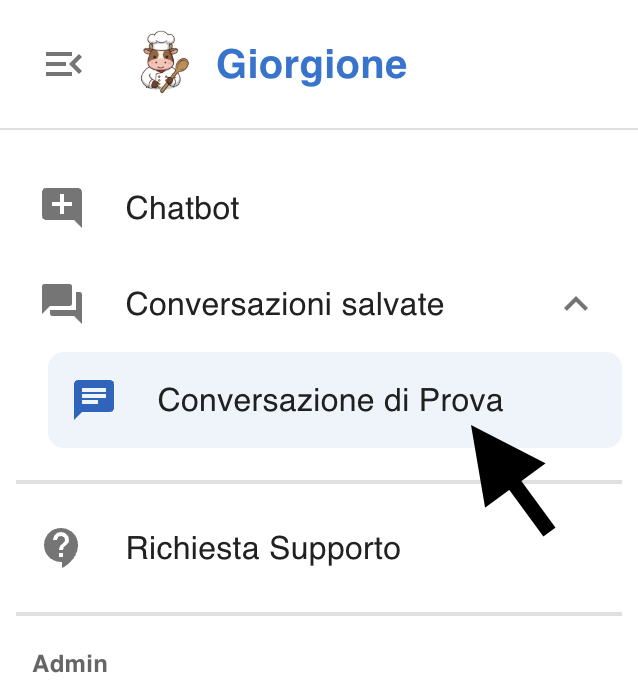
\includegraphics[width=\textwidth]{./img/laterale2.png}
    \end{subfigure}
    \caption{Menù laterale}
\end{figure}
L'utente si trovera quindi di fronte a una schermata composta da diversi elementi:
\begin{figure}[h!]
    \centering
    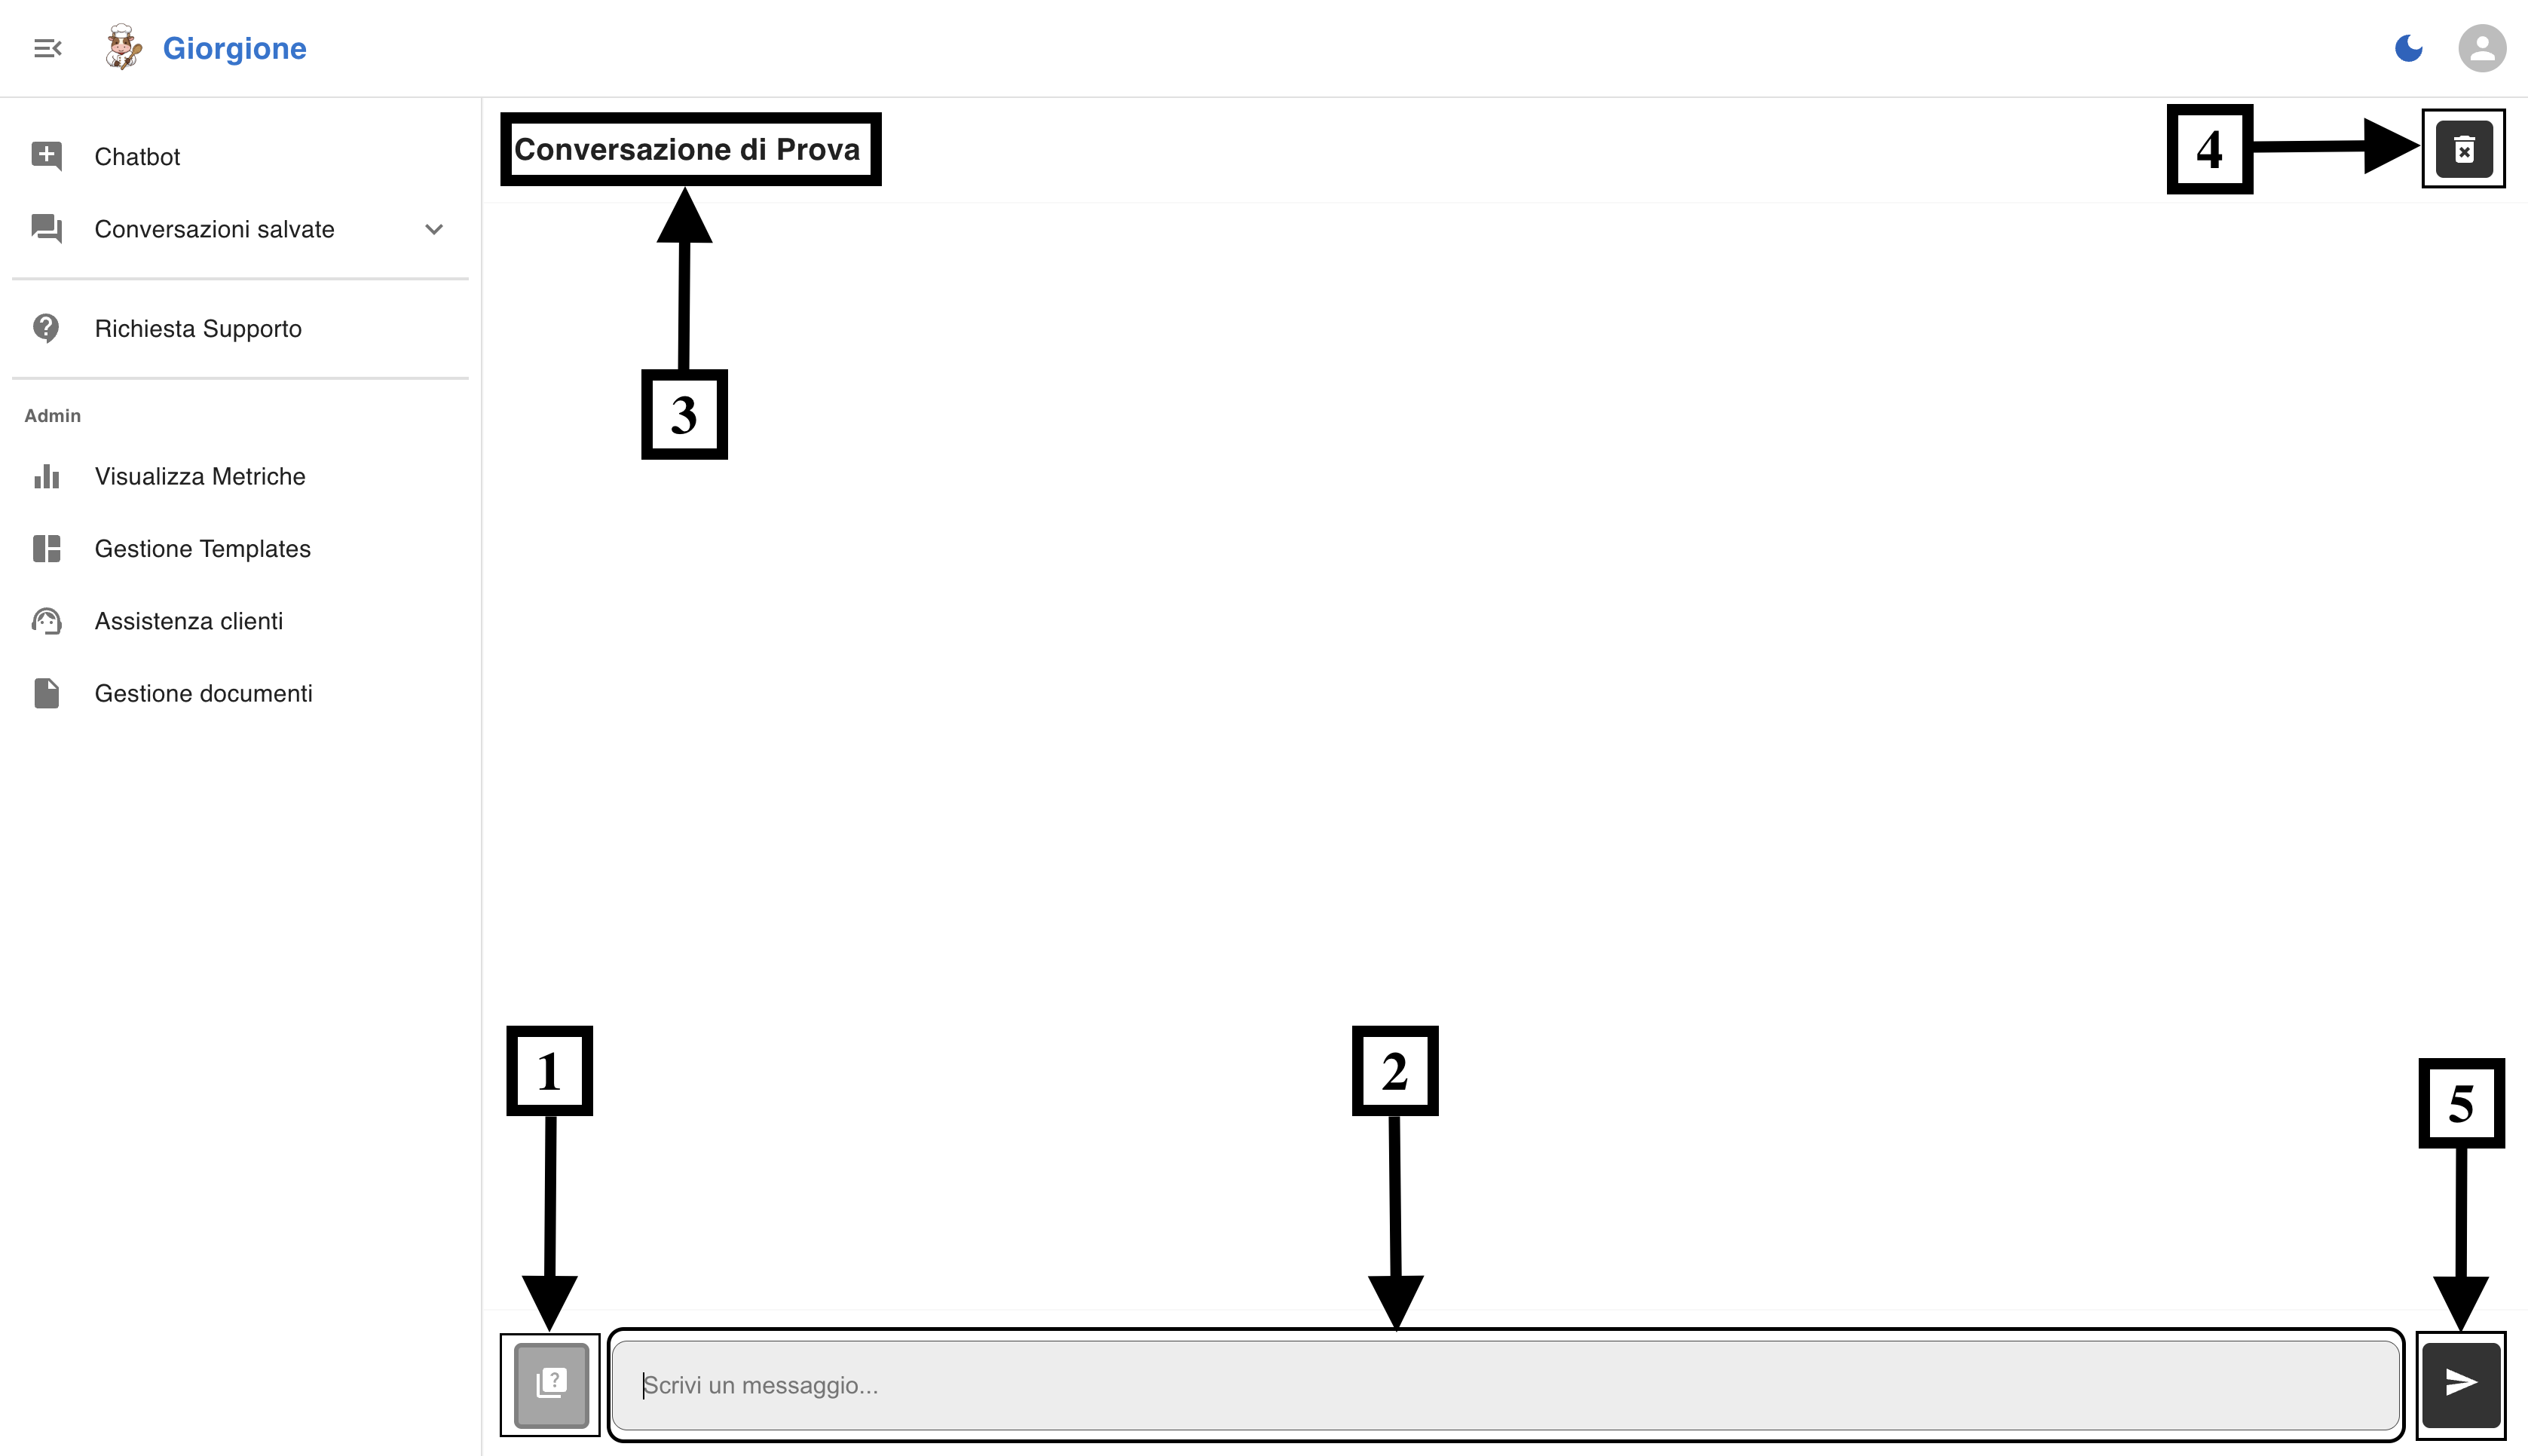
\includegraphics[width=\textwidth]{./img/SchermataChat1.png}
    \caption{Schermata della chat}
    \label{fig:schermata-chat}
\end{figure}
\newpage
Facendo riferimento alla figura~\ref{fig:schermata-chat} infatti l'utente troverà un bottone per selezionare una domanda templetizzata (\textit{qui segnato con il numero 1}), cliccato il bottone sarà presente selezionare la domanda e inviarla all'assistente virtuale come mostrato in figura~\ref{fig:domanda templetizzata}.
\begin{figure}[htbp]
    \centering
    \begin{tikzpicture}
        % Inserisci le immagini
        \node[anchor=east,inner sep=0] (img1) at (0,0) {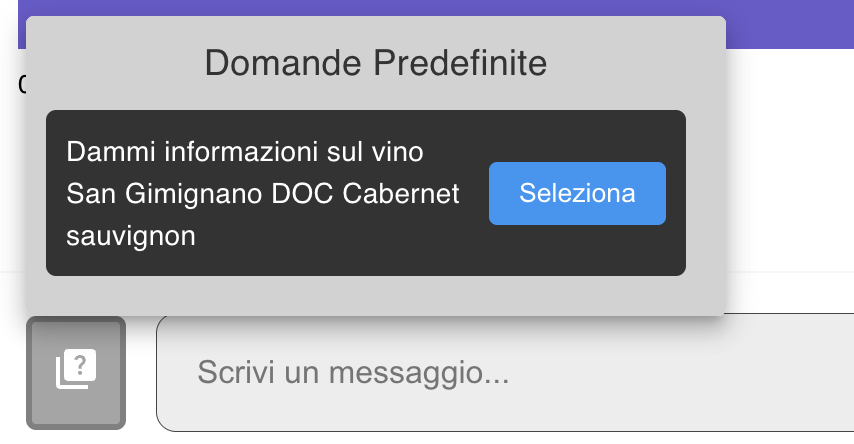
\includegraphics[width=0.4\textwidth]{img/SelettoreTemplate1.png}};
        \node[anchor=west,inner sep=0] (img2) at (2,0) {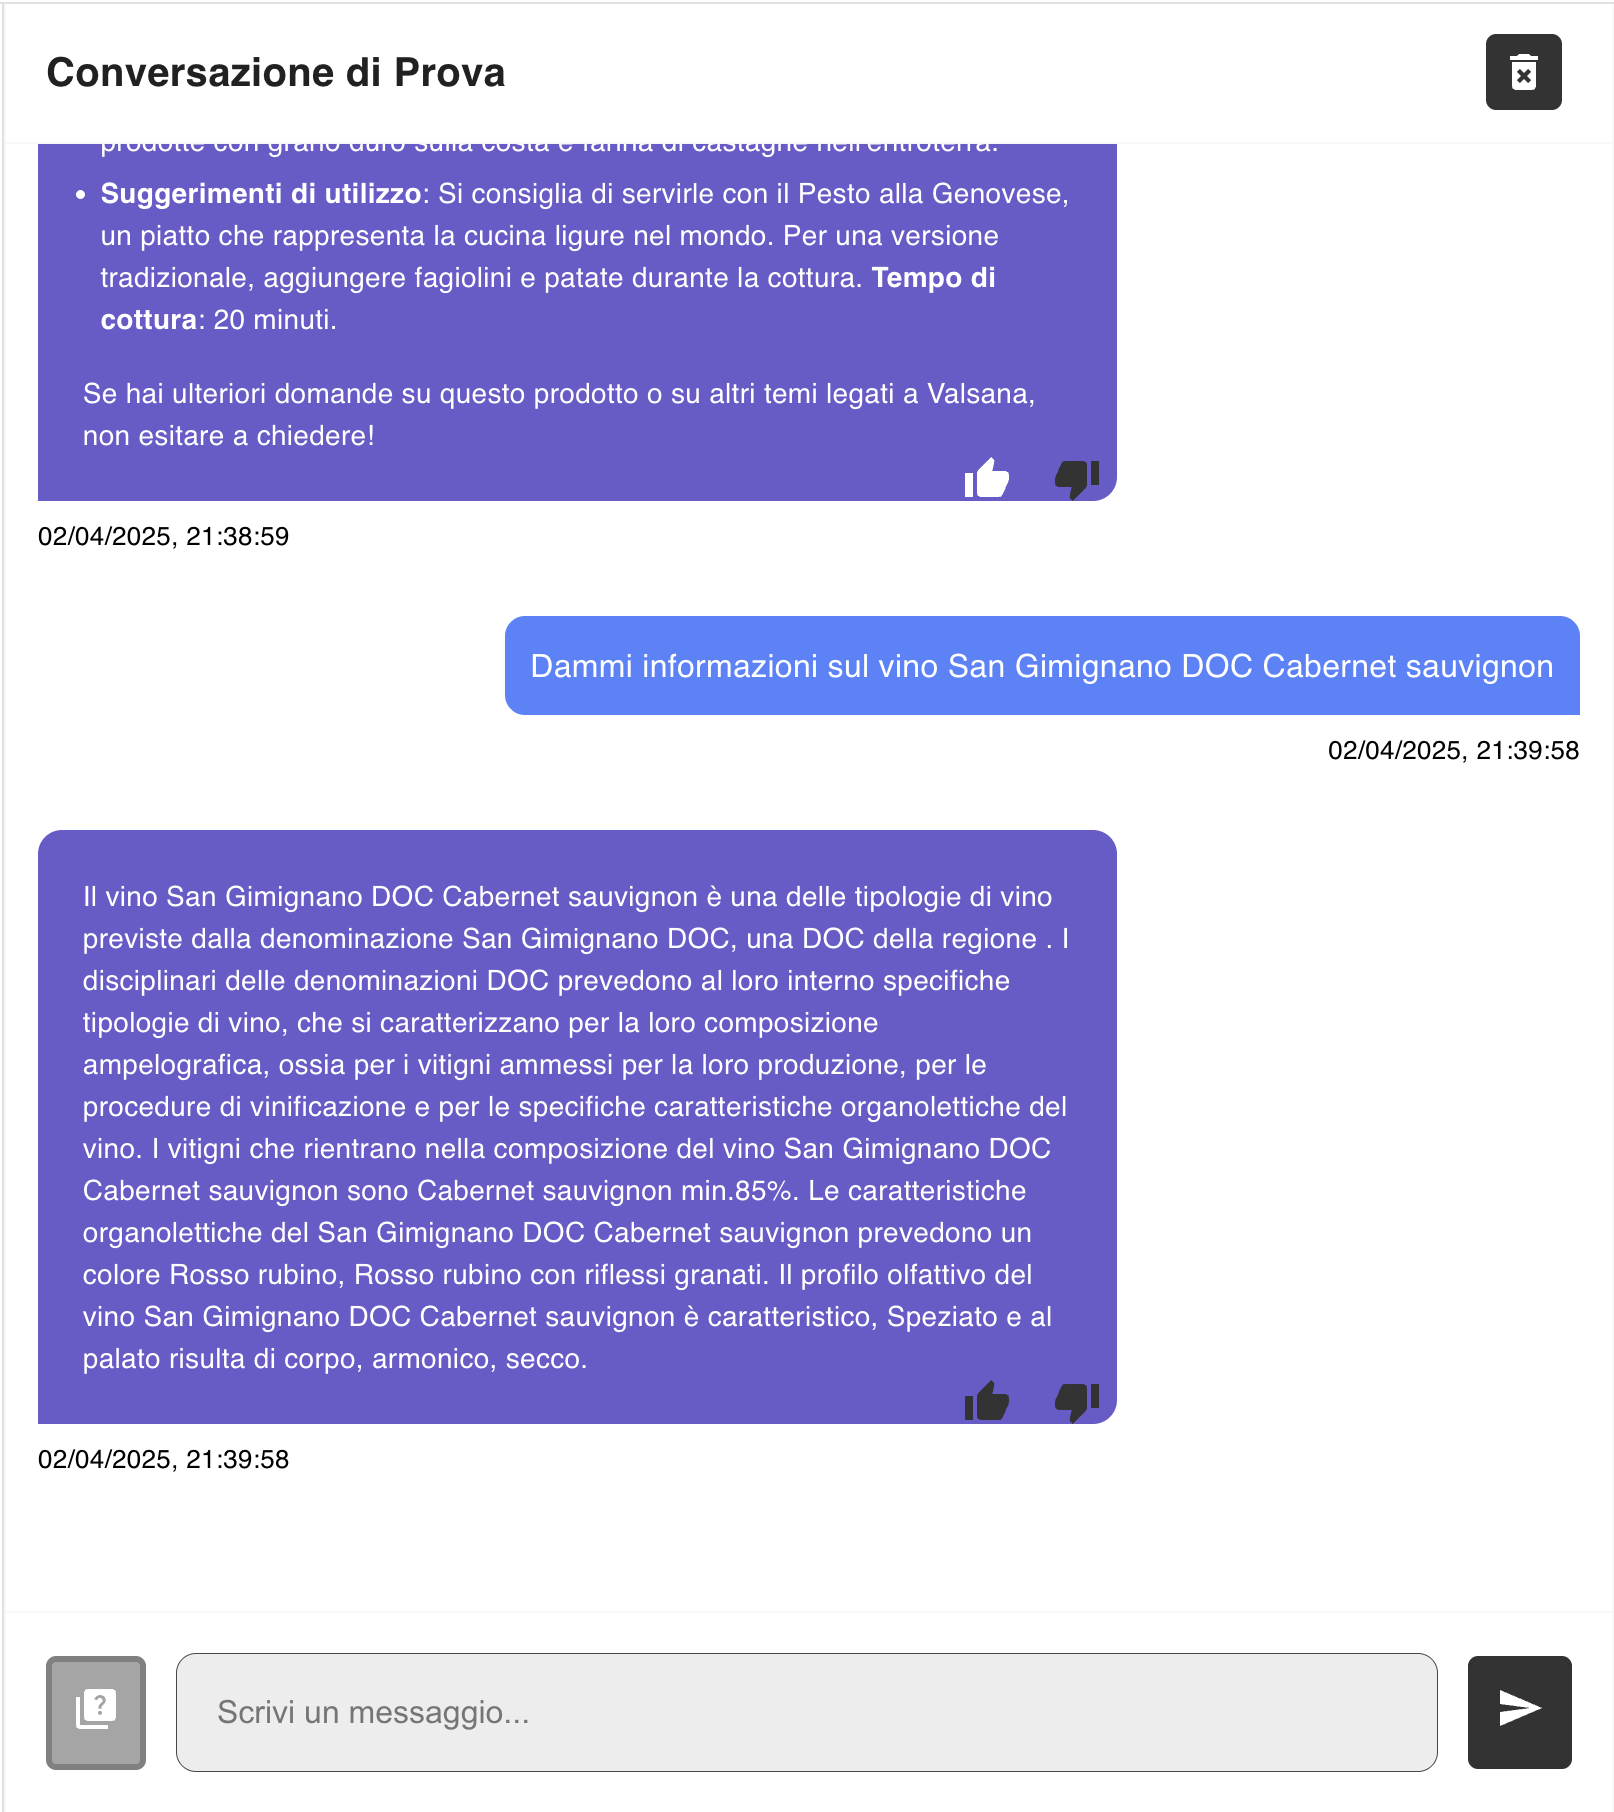
\includegraphics[width=0.4\textwidth]{img/SelettoreTemplate2.png}};
        
        % Disegna una freccia
        % Disegna una freccia dritta orizzontale
        \draw[->, thick] (img1.east) -- (img2.west);
        \end{tikzpicture}
        \caption{Seleziona domanda templetizzata}
        \label{fig:domanda templetizzata}
\end{figure}
\\
Il punto numero 2 indica invece la casella di testo dove l'utente potrà scrivere il proprio messaggio da inviare al bot.
Il punto numero 3 indica il nome della conversazione precedentemente scelto nella schermata iniziale. Il punto numero 4 indica un bottone che permette di eliminare la chat premendolo apparirà un pop-up che chiede cortesemente all'utente se è sicuro di voler eliminare la conversazione figura~\ref{fig:elimina-chat}:
\begin{figure}[h!]
    \centering
    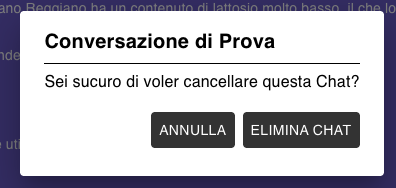
\includegraphics[width=0.5\textwidth]{./img/eliminaChat.png}
    \caption{Elimina chat}
    \label{fig:elimina-chat}
\end{figure}
\\
Il punto numero 5 in figura~\ref{fig:schermata-chat} è il pulsante invio che permette di mandare un messaggio al nostro assistente virtuale. Bisogna dire tuttavia che è possibile inviare un messaggio solo se del testo è presente nella casella di testo (\textit{punto 2 in figura~\ref{fig:schermata-chat}}) e che non è necessario cliccare sul pulsante in quanto è possibile premere direttamente invio sulla tastiera.
\\
Inviato un messaggio questo apparirà nella parte destra della schermata come avviene nelle più famose chat di messaggistica (fare riferimento a figura~\ref{fig:Elaborazione} punto 6), e verrà mostrato il messaggio e la data e l'ora dell'invio.
Nella parte sinistra l'utente potrà osservare il nostro Assistente virtuale Giorgione elaborare il messaggio per soddisfare la richiesta dell'utente (punto 7 figura~\ref{fig:Elaborazione}).
\begin{figure}[h!]
    \centering
    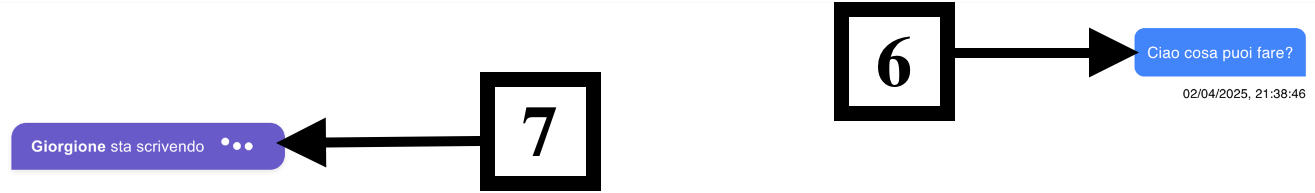
\includegraphics[width=\textwidth]{./img/SchermataChat2.png}
    \caption{Elaborazione del messaggio}
    \label{fig:Elaborazione}
\end{figure}
\\
Una volta mandato il messaggio esso sarà visualizzabile come mostrato in figura~\ref{fig:Visualizzazione Risposta} punto 8, e l'utente potrà decidere opzionalmente se è soddisfatto della risposta data dal bot di fornire una valutazione booleana indicata da un pollice in su e pollice in giù (\textit{figura~\ref{fig:Visualizzazione Risposta} punto 9}):
\begin{figure}[h!]
    \centering
    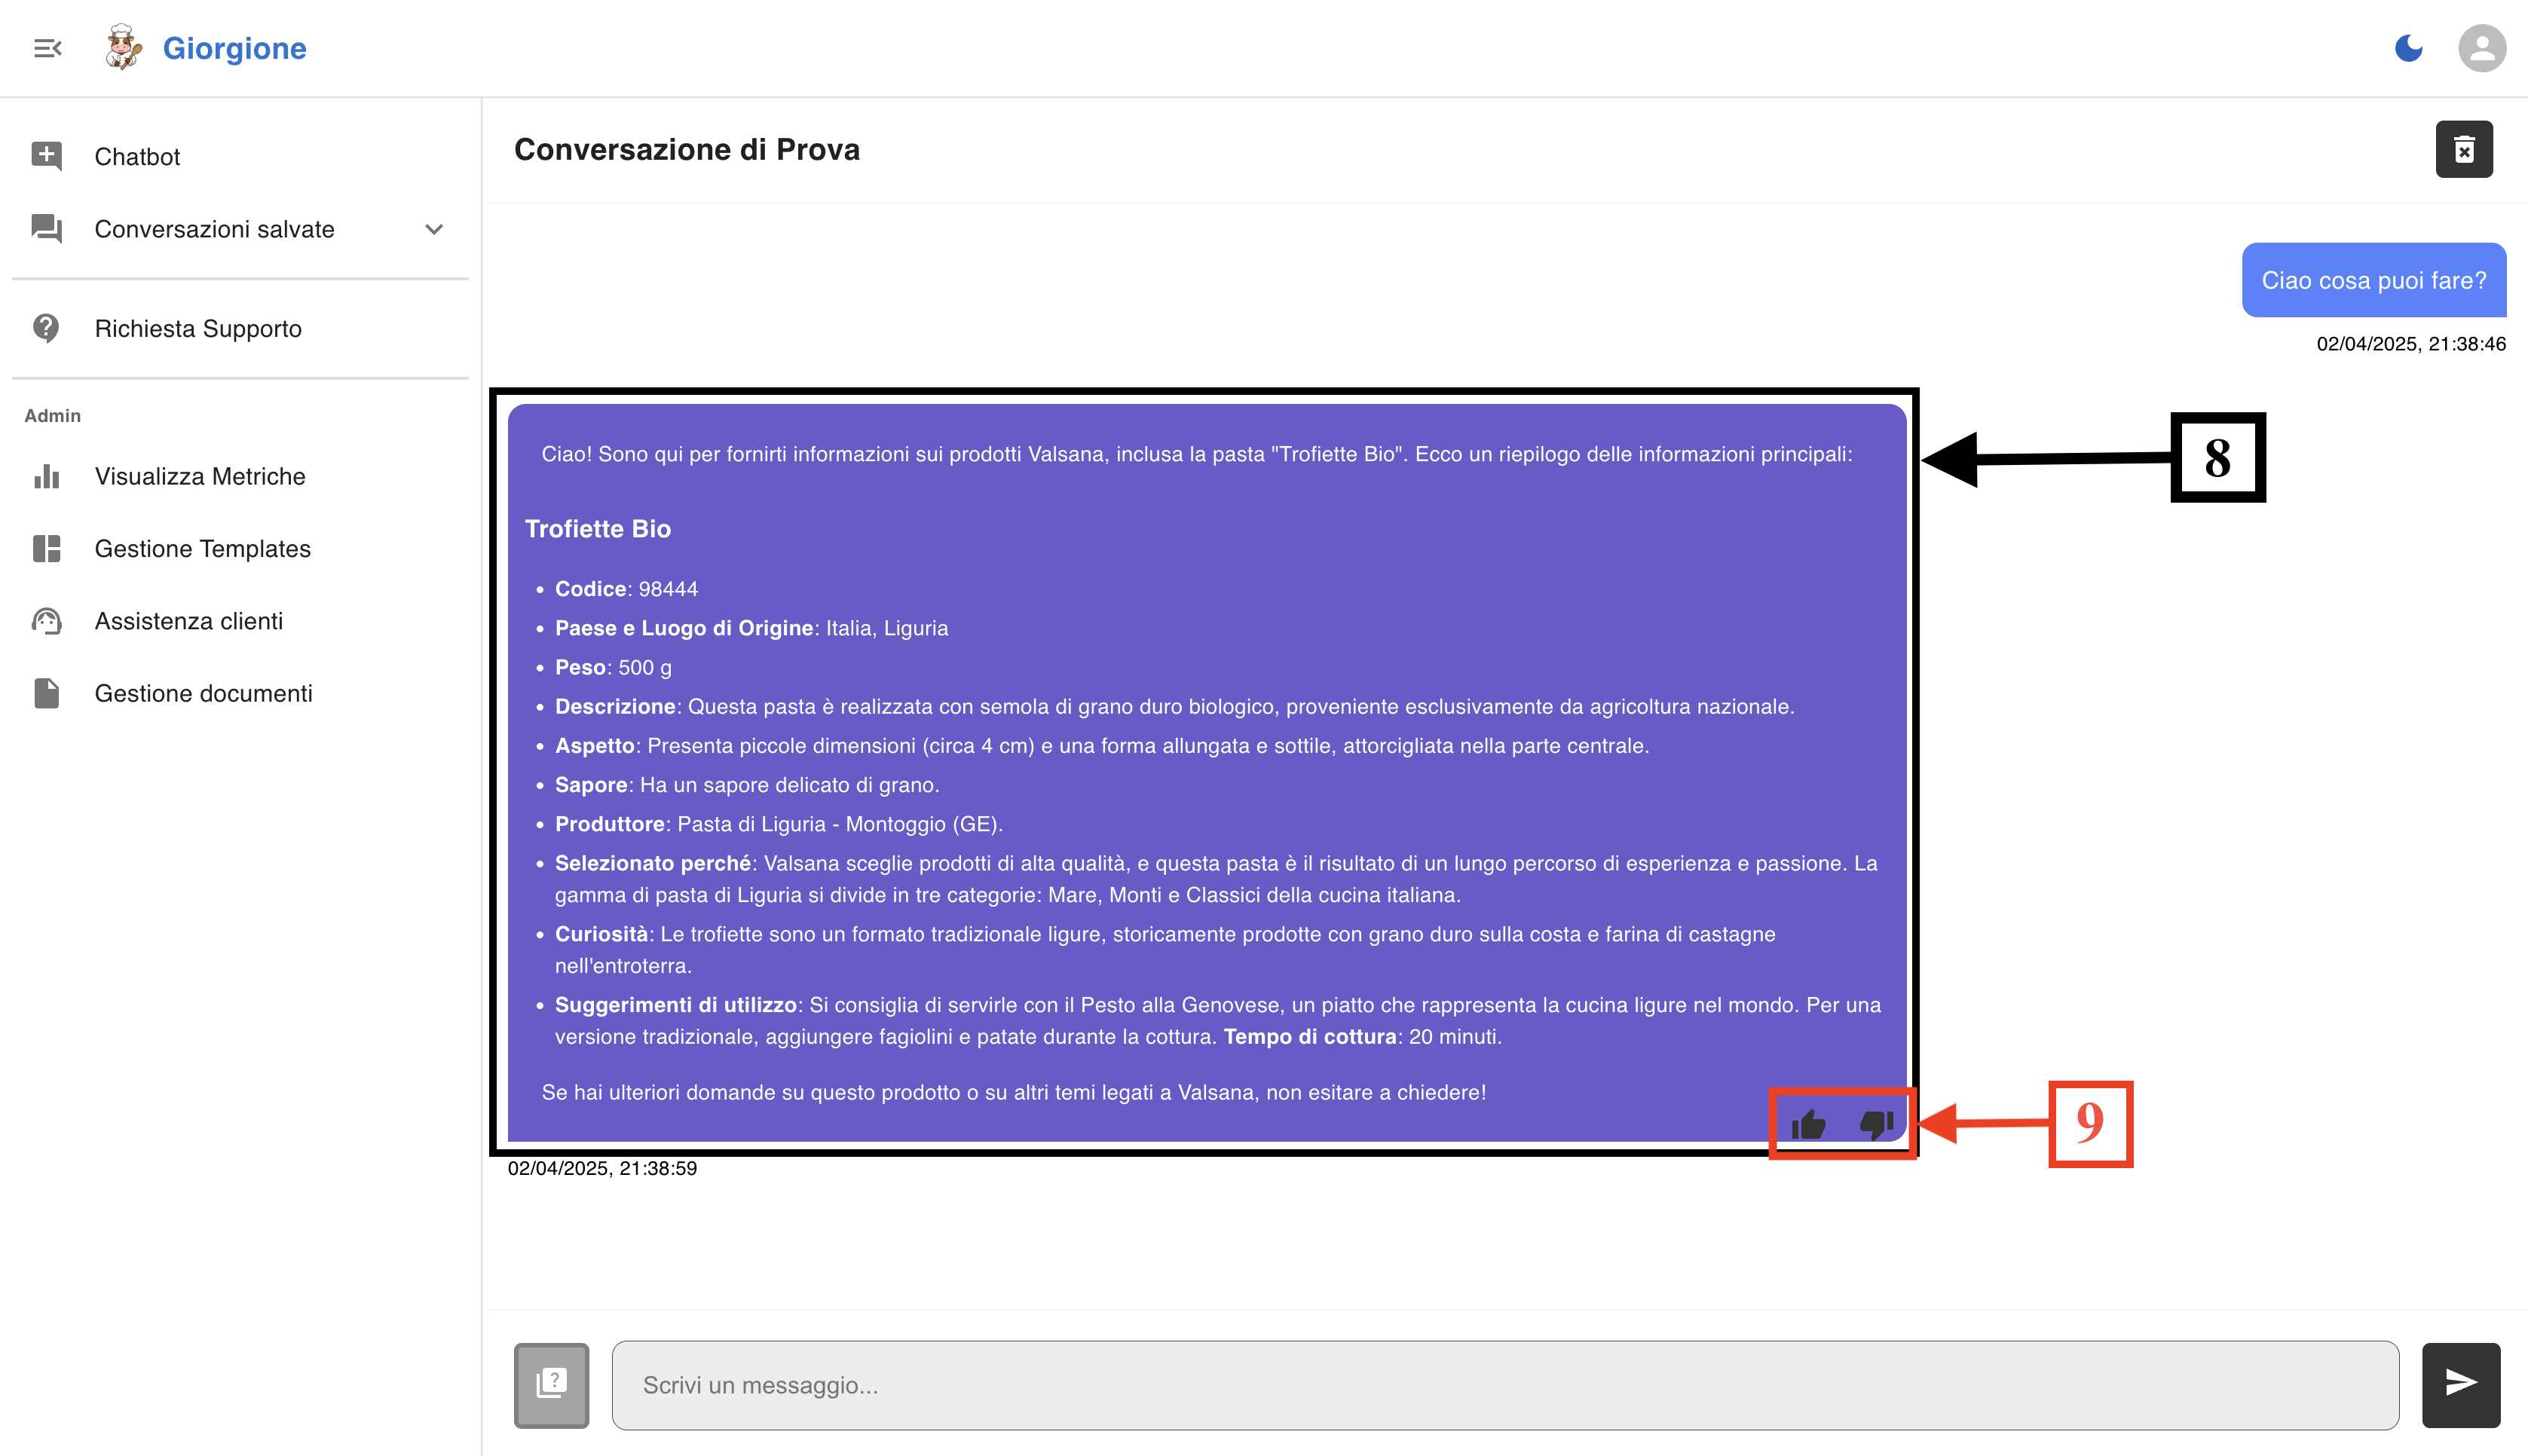
\includegraphics[width=\textwidth]{./img/SchermataChat3.png}
    \caption{Visualizzazione Risposta}
    \label{fig:Visualizzazione Risposta}
\end{figure}
L'utente è notificato dalla scelta dall'illuminazione di uno dei 2 bottoni come mostrato in figura~\ref{fig:likedislike}
\begin{figure}[h!]
    \centering
    \begin{subfigure}{0.2\textwidth}
        \centering
        
\includegraphics[width=\textwidth]{./img/like.png}
        \caption{Caso in cui l'utente scelga like}
    \end{subfigure}
    \hspace{0.05\textwidth}
    \begin{subfigure}{0.2\textwidth}
        \centering
        
\includegraphics[width=\textwidth]{./img/dislike.png}
        \caption{Caso in cui l'utente scelga dislike}
    \end{subfigure}
    \caption{Feedback Risposta}
    \label{fig:likedislike}
\end{figure}

\newpage

\subsubsection{Pagina di Richiesta di Supporto}
Selezionando dal menù laterale la voce "Richiesta Supporto" (fig~\ref{fig:Pagina di Assistenza} pt.1). L'utente si troverà davanti ad una pagina dove potrà inviare un messaggio all'admin in caso di problemi.
Una richiesta dovrà essere composta da un Oggetto inseribile nella casella di testo (fig~\ref{fig:Pagina di Assistenza} pt.2), una descrizione (fig~\ref{fig:Pagina di Assistenza} pt.3).\\
Una volta compilati l'utente può inviare il messaggio cliccando sul bottone invia indicato in fig~\ref{fig:Pagina di Assistenza} pt.4, e successivamente verrà notificato dell'invio riuscito o non riuscito come mostrato in fig~\ref{fig:InvioRiuscito} (\textit{Ci riserviamo di mostrare solo l'invio riuscito}).
\begin{figure}[h!]
    \centering
    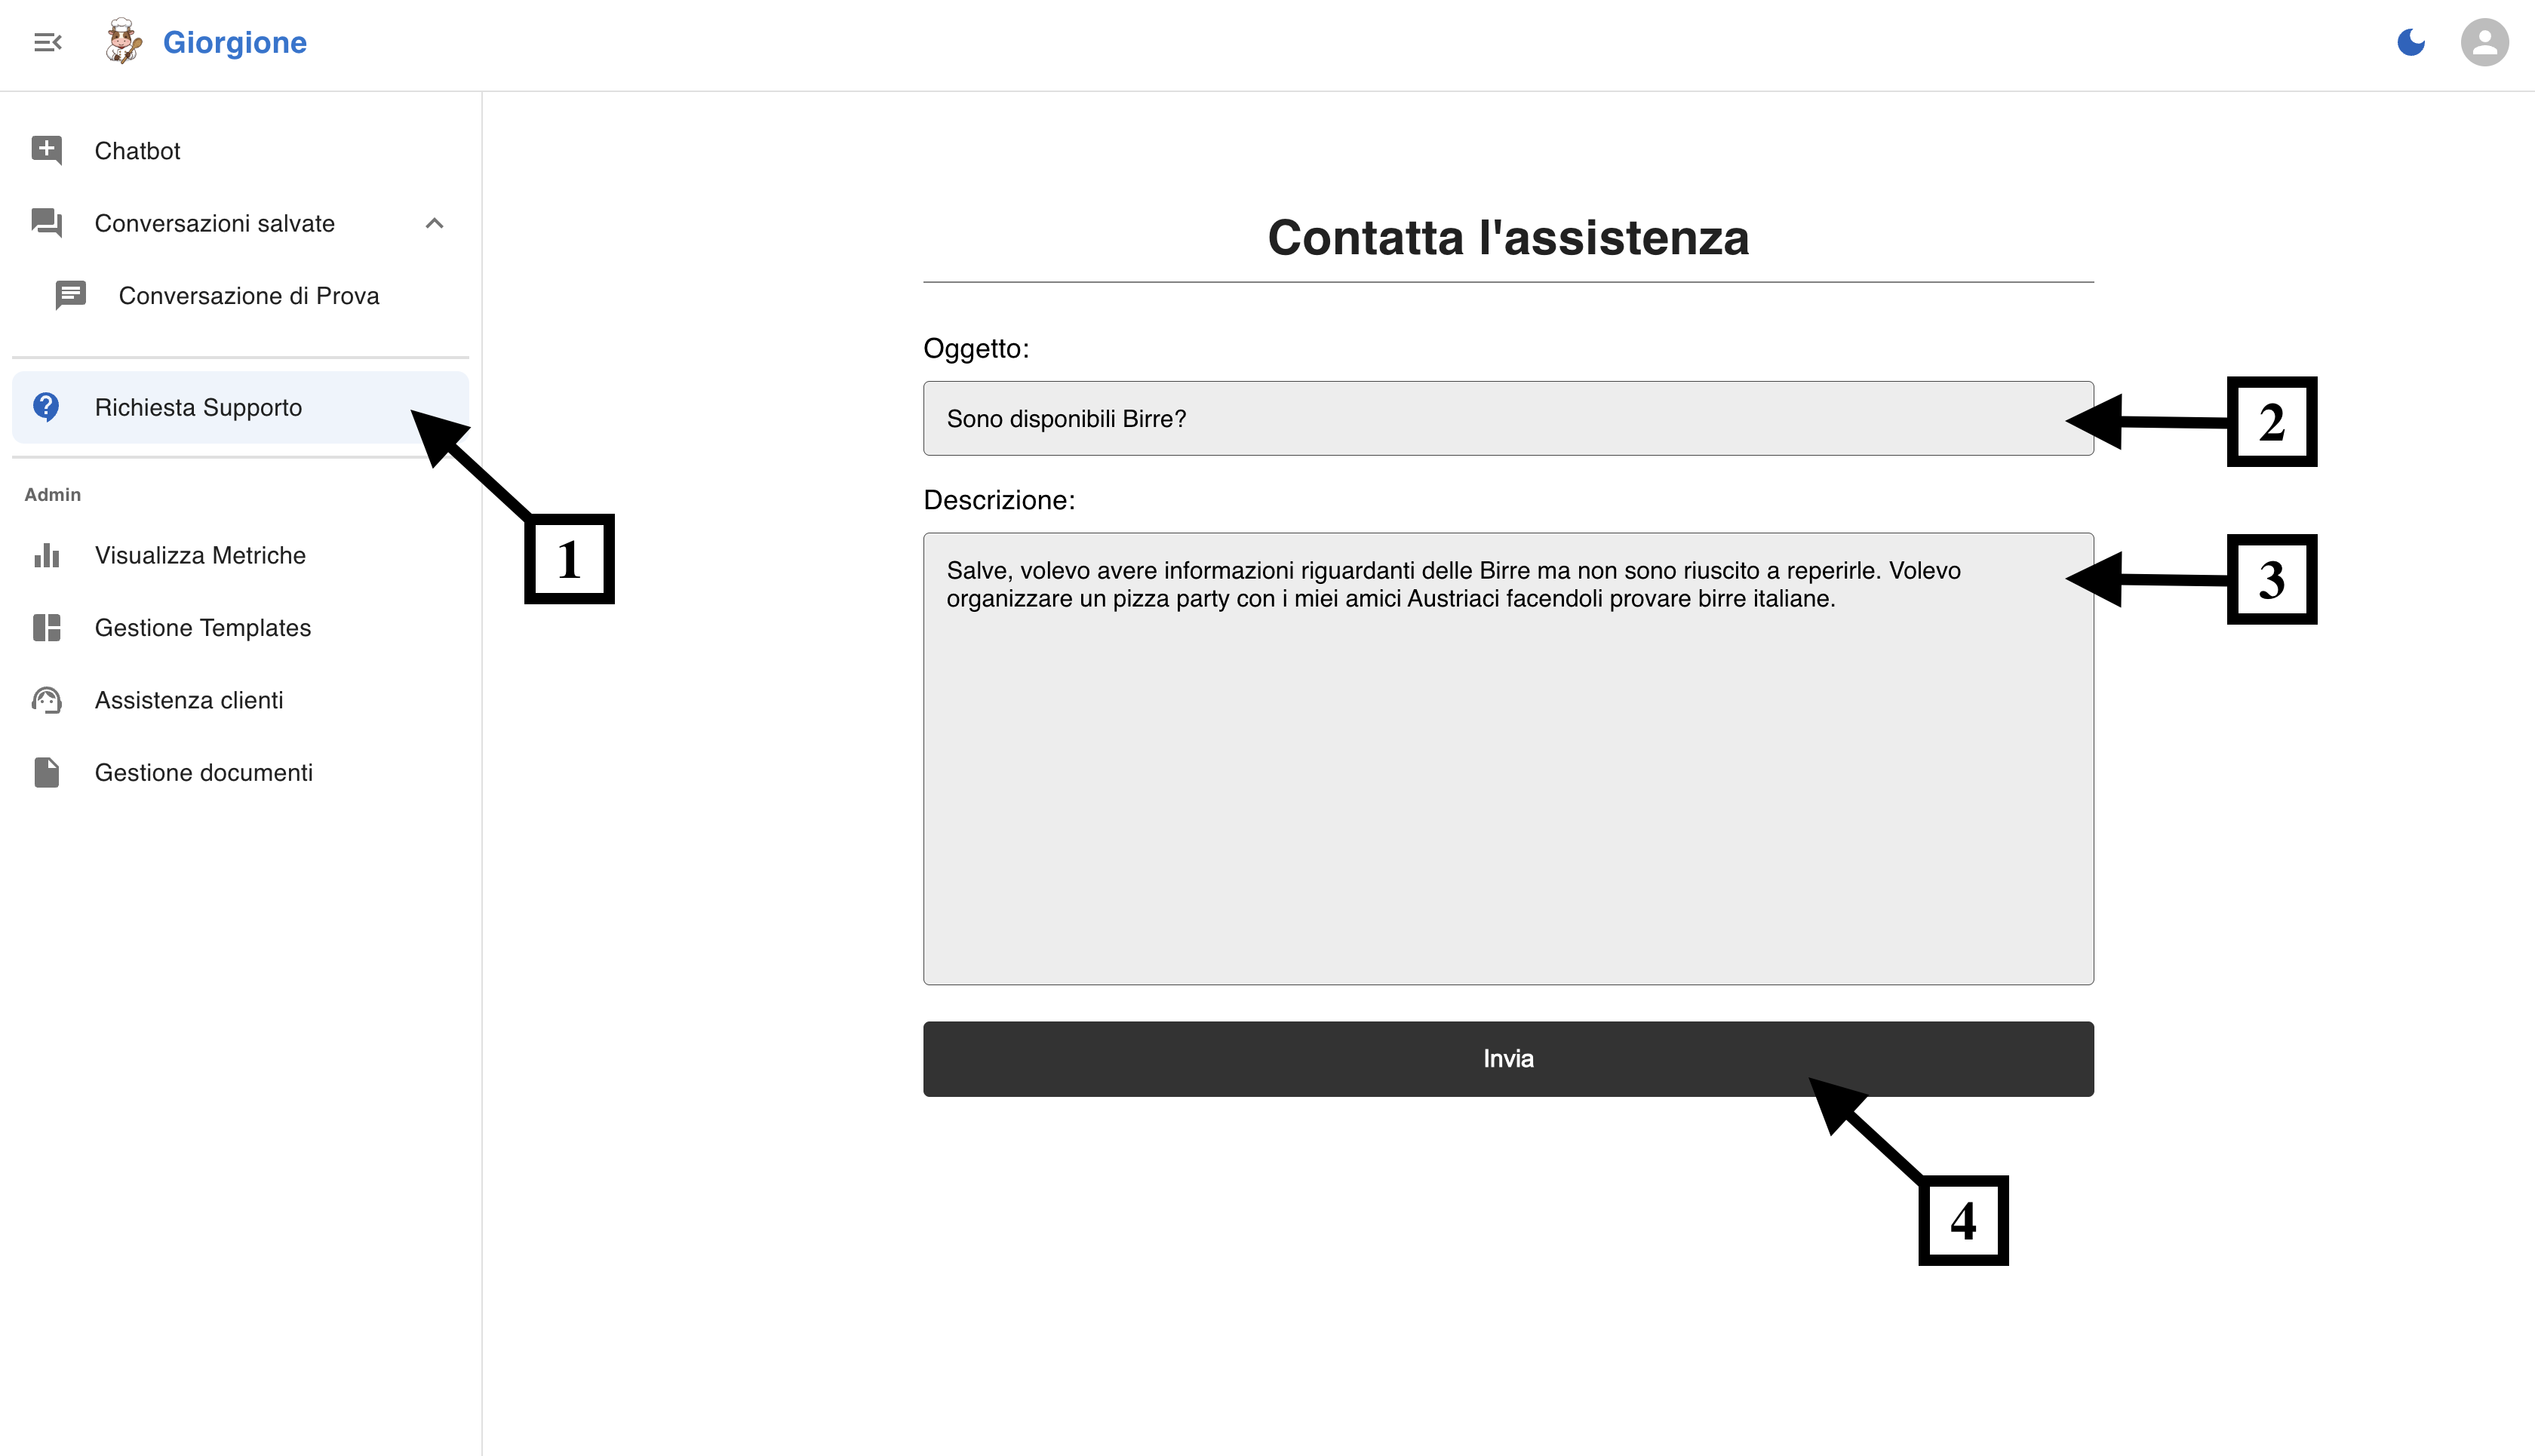
\includegraphics[width=\textwidth]{./img/RichiestaAssistenza1.png}
    \caption{Pagina di Assistenza}
    \label{fig:Pagina di Assistenza}
\end{figure}
\begin{figure}[h!]
    \centering
    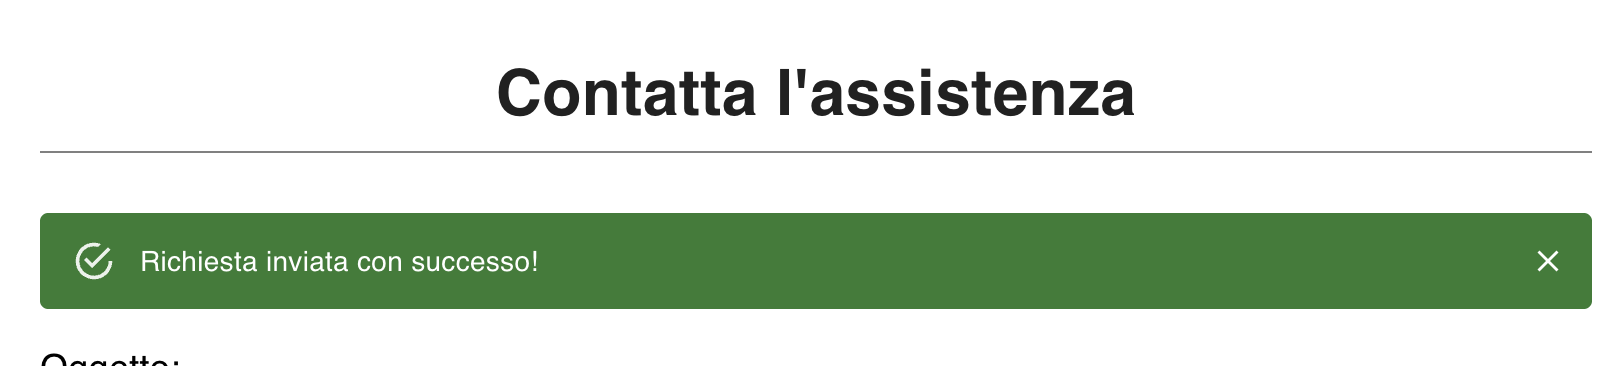
\includegraphics[width=0.8\textwidth]{./img/RichiestaAssistenza2.png}
    \caption{Invio Richiesta Assistenza Riuscita}
    \label{fig:InvioRiuscito}
\end{figure}

\subsection{Pagine riservate all'admin}
In questa sezione mostriamo le pagine riservate all'admin.

\subsubsection{Visualizza Metriche}
L'admin cliccando dal menù laterale su Visualizza Metriche vedrà una Dashboard dove visualizzerà con valori numerici i like e i dislike delle conversazioni e il numero di messaggi totali gestiti dal Database.
\begin{figure}[h!]
    \centering
    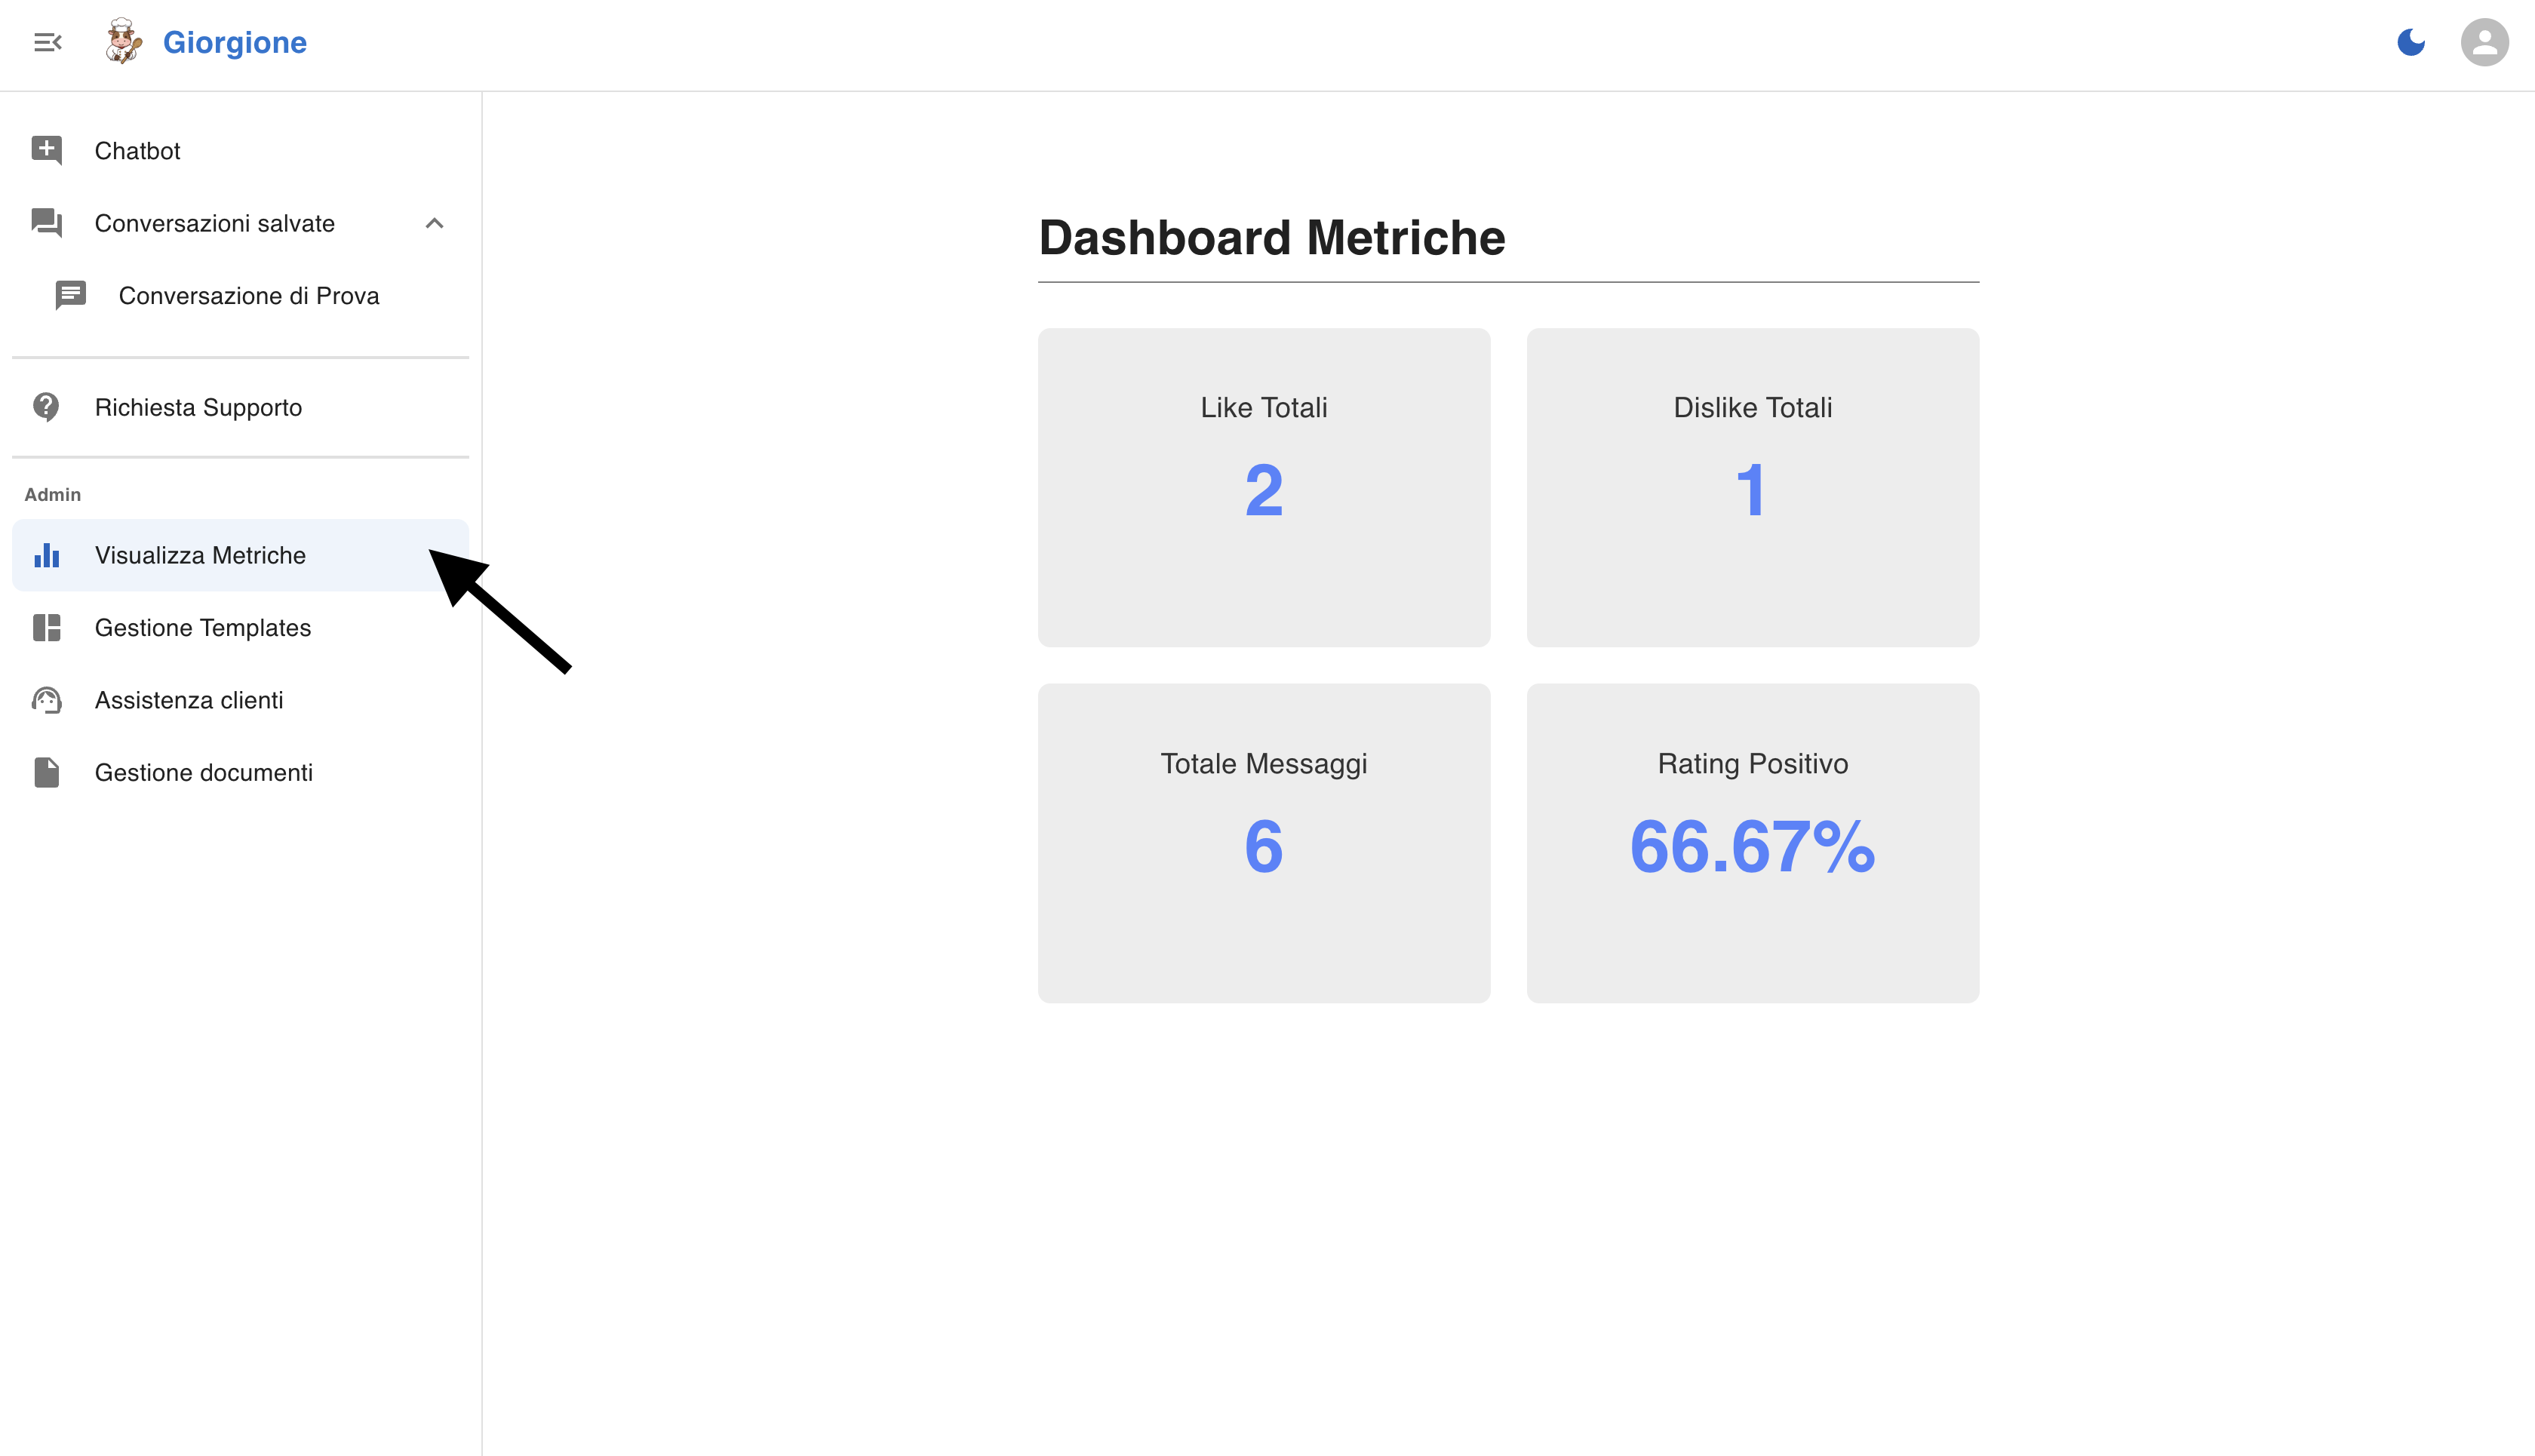
\includegraphics[width=\textwidth]{./img/visualizzaMetriche.png}
    \caption{Dashboard Metriche}
    \label{fig:Metriche}
\end{figure}

\subsubsection{Gestione Template}
Selezionado dal menù laterale (fig~\ref{fig:Template} pt.1) accediamo alla pagina di gestione dei template. Qui è possibile visualizzare i template precedentemente inseriti dall'admin, aggiungerne di nuovi, modificarli ed eliminarli.
\begin{figure}[h!]
    \centering
    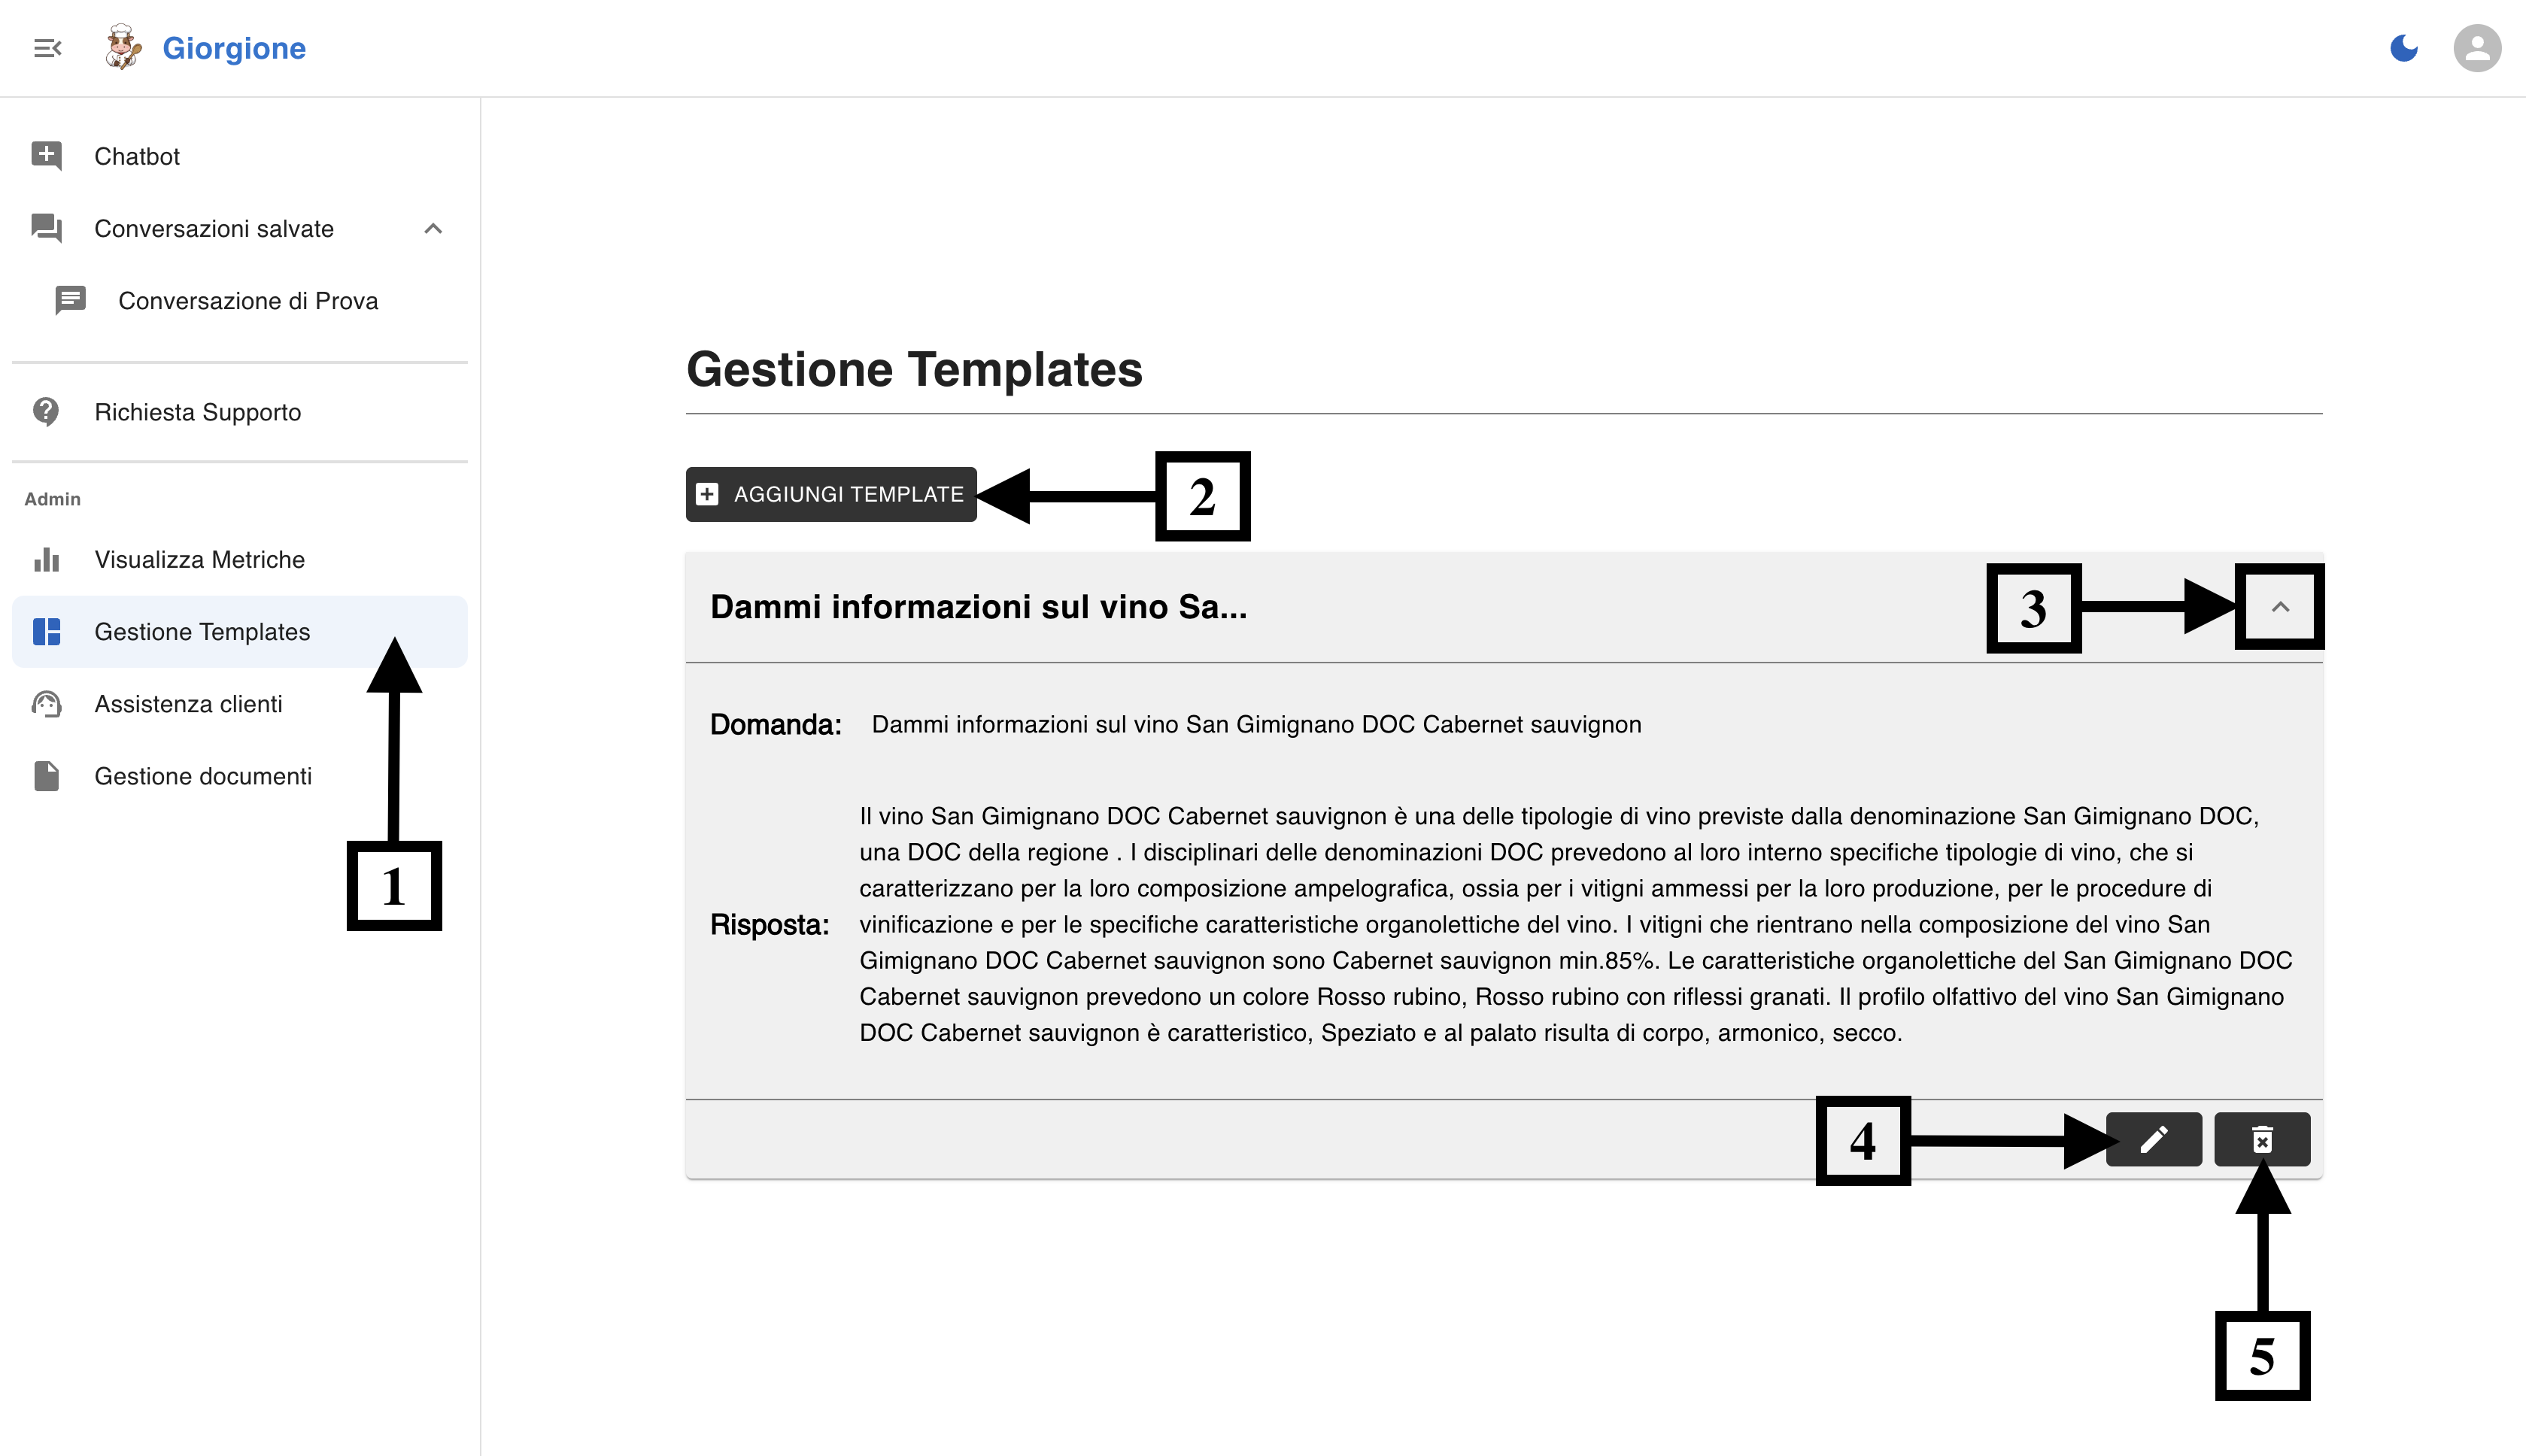
\includegraphics[width=\textwidth]{./img/GestioneTemplate.png}
    \caption{Gestione Template}
    \label{fig:Template}
\end{figure}
Per aggiungere un template basterà cliccare sul pulsante aggiungi template (fig~\ref{fig:Template} pt.2) che aprirà il pop-up mostrato in fig~\ref{fig:addTemplate} dove sarà possibile inserire la domanda e la risposta.
\begin{figure}[h!]
    \centering
    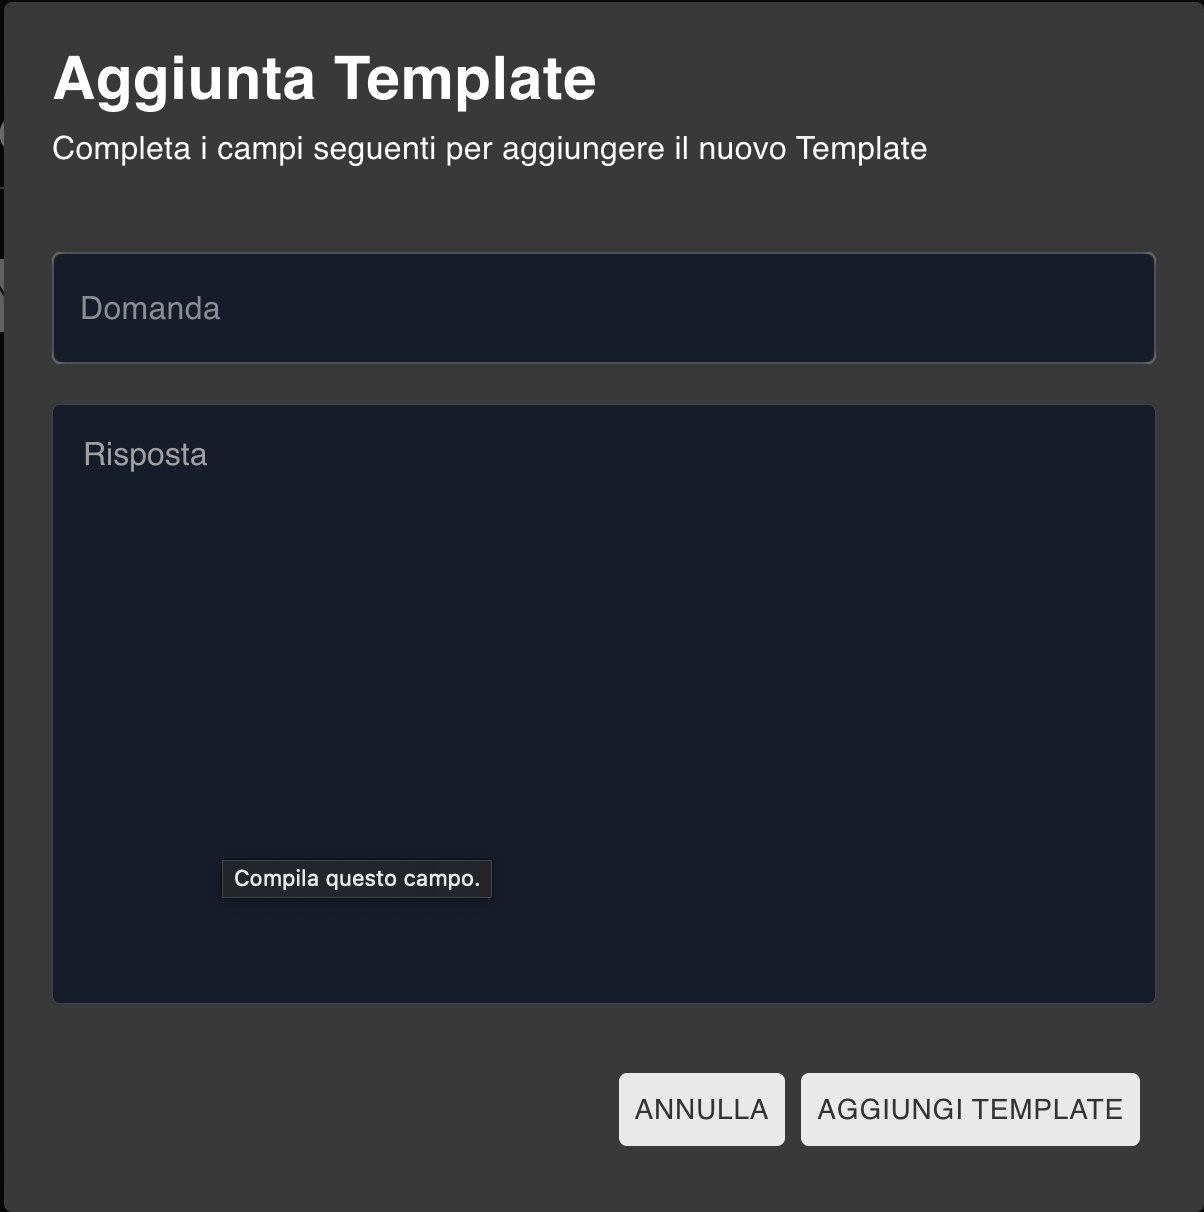
\includegraphics[width=0.4\textwidth]{./img/AggiungiTemplate.png}
    \caption{Aggiungi Template}
    \label{fig:addTemplate}
\end{figure}
Per visualizzare l'intero template e non solo il nome è possibile cliccare sul bottone mostrato in fig~\ref{fig:Template} pt.3 che aprirà una tendina dove verrà visualizzata l'intera domanda e l'intera risposta. Verranno inoltre mostrati il pulsanti di "modifica template" (fig~\ref{fig:Template} pt.4) ed "elimina template" (fig~\ref{fig:Template} pt.5). Se questi ultimi dovessero essere cliccati appariranno i pop-up mostrati in figura~\ref{fig:pop-up modifica ed elimina}.
\begin{figure}[h!]
    \centering
    \begin{subfigure}{0.2\textwidth}
        \centering
        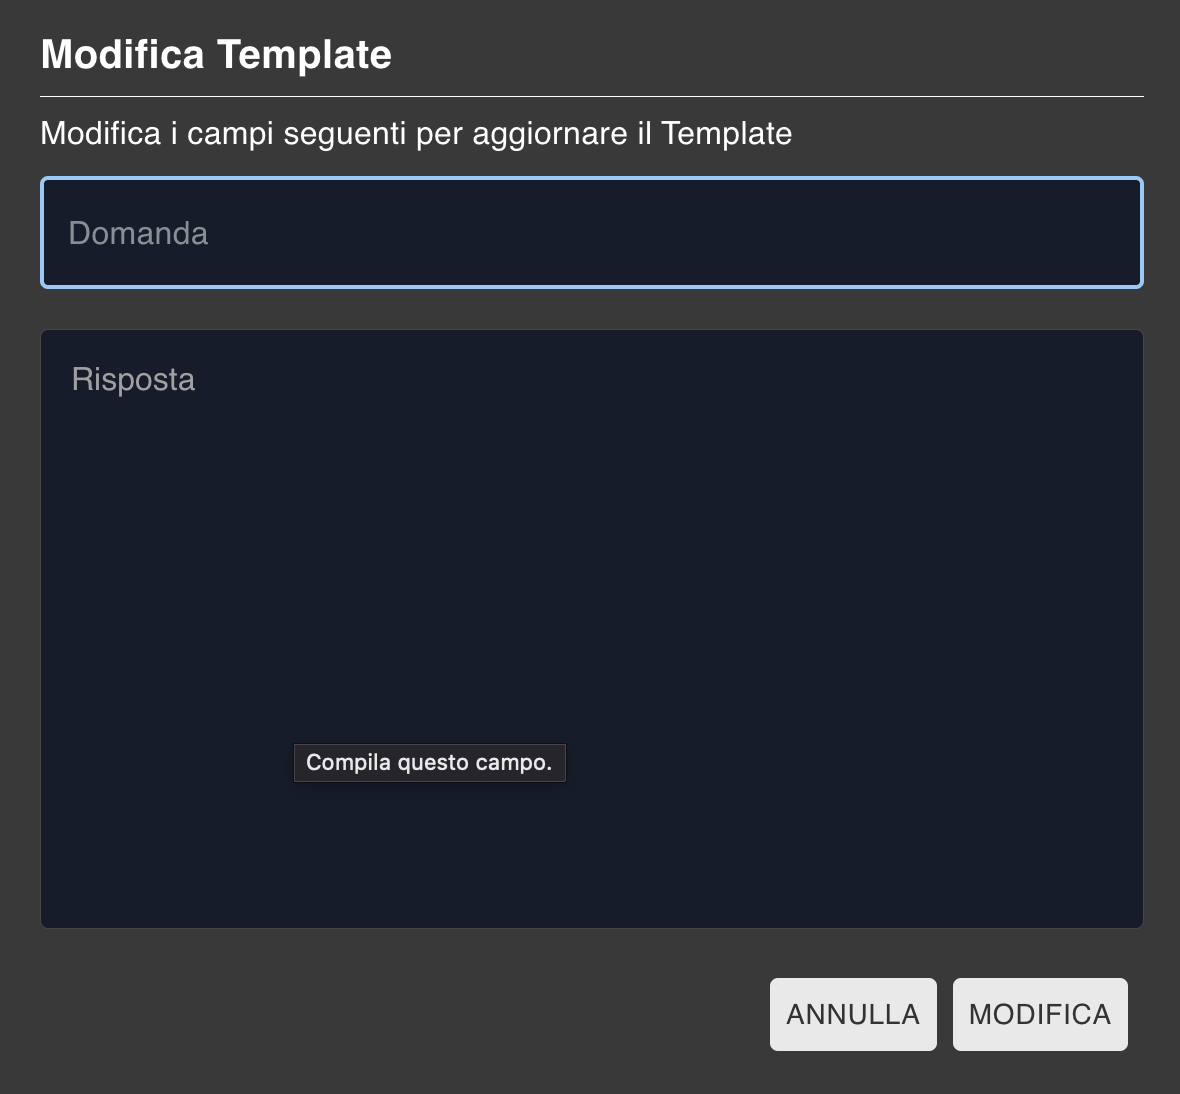
\includegraphics[width=0.7\textwidth]{./img/ModificaTemplate.png}
        \caption{ModificaTemplate}
    \end{subfigure}
    \hspace{0.05\textwidth}
    \begin{subfigure}{0.2\textwidth}
        \centering
        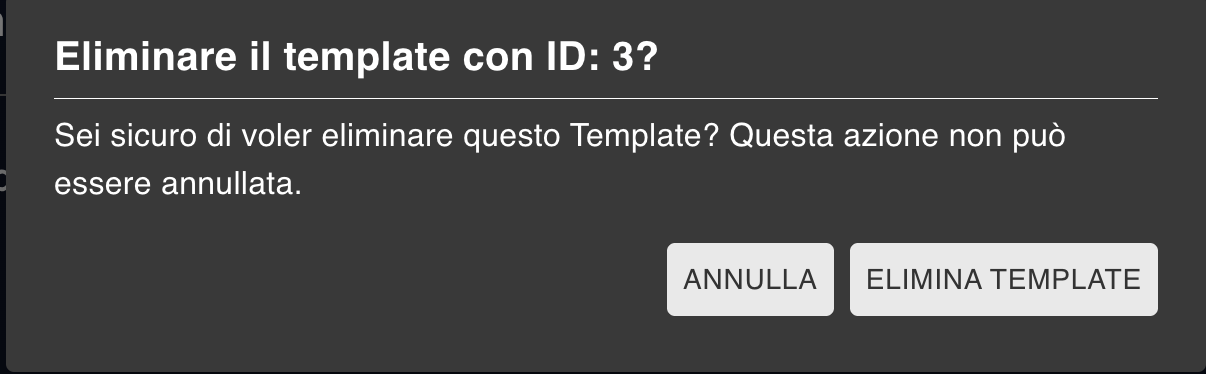
\includegraphics[width=\textwidth]{./img/EliminaTemplate.png}
        \caption{Elimina Template}
    \end{subfigure}
    \caption{Modifica Template ed Elimina Template}
    \label{fig:pop-up modifica ed elimina}
\end{figure}

